\section{Detailed control design for agreed plant section}
\label{sec:subsec}

\subsection{Description of sub-section}
The agreed subsection has a gaseous \ch{H2} feed and liquid feed consisting of methanol and o-nitrotoluene entering the top of a trickle bed reactor (R201). The streams are preheated electric heaters H201 and H202. The reactor has a gaseous effluent which is split into a recycle and purge stream. The liquid effluent enters a packed distillation column (S201), where methanol is separated from the heavier organics. The methanol-rich vapour from the column is partially condensed and split into a gaseous and liquid product in a reflux drum (S204), while the bottoms stream containing valuable o-toluidine product is sent to downstream purification units.

\subsection{Degree of freedom analysis}

\begin{wraptable}{r}{0.55\linewidth}
\centering
    \caption{Degree of freedom analysis}
    \label{tab:dof}
\begin{tabular}{@{}lllll@{}}
\toprule
Total number of process streams (+) & 28 &  &  &  \\ \midrule
Sum of restraining numbers (-)      & 11 &  &  &  \\
Sum of mechanical agitators (+)     & 2  &  &  &  \\
Redundancies (-)                    & 3  &  &  &  \\
Control degrees of freedom          & 16 &  &  &  \\ \bottomrule
\end{tabular}
\end{wraptable}

To determine the number of variables that can be simultaneously manipulated to maintain stable operation in our sub-section, a degree of freedom analysis was carried out. A thorough analysis involves subtracting the total number of variables from the total number of equations in a dynamic model of each process unit, however creating such models are often impractical and error-prone for complex plants with specialised units. Instead, the simpler and straightforward method presented by \textcite{} showed that there are a maximum of 14 variables that could be manipulated for control (see Table \ref{tab:dof}).

\subsection{Key control loops}
\Cref{tab:controls} shows a summary of the control loops in the plant sub-section. A total of 14 variables were controlled using feedback, feedforward, cascade, ratio and inferential control in order to ensure stable operation of the units in the sub-section.

\begin{table}[h]
\centering
    \caption{Summary of control loops}
    \label{tab:controls}\footnotesize
\adjustbox{max width=\textwidth}{
\begin{tabular}{p{3cm}|p{3cm}|p{4cm}|p{5cm}|p{6cm}}
\toprule
\textbf{Unit}                               & \textbf{Controlled Variable}                & \textbf{Manipulated Variable}                           & \textbf{Sensor/Actuator}                                                   & \textbf{Control Strategy}                                                                                                            \\ \midrule
\multirow{7}{*}{Reactor (R201)}             & Temperature of reactor                      & Cooling water flowrate in reactor jacket                & Temperature sensor (TT-201) / Flow control valve (FCV-201)                 & Feedforward control mitigates temperature disturbances and cascade   control counters flow disturbances in cooling water.            \\
                                            & Pressure of reactor                         & Pressure of the fresh hydrogen                          & Pressure sensor (PT-201) / Pressure control valve (PCV-202)                & Feedforward control mitigates disturbances in upstream fresh H­2 pressure and recycle H2 pressure.                                   \\
                                            & Ratio of reactants                          & Flowrate of fresh methanol                              & Flow sensors (FT-202, FT-203) / Pump speed (P201)                          & Ratio control ensures the H2 and liquid feed enter the reactor in fixed proportions.                                                 \\
                                            & Composition of gas feed to reactor          & Flowrate of purge                                       & Composition analyser (AT-203) / Flow control valve (FCV-203)               & Cascade control allows composition to be manipulated using the purge   flowrate which is a slave control to smooth any disturbances. \\
                                            & Level                                       & Flowrate of reactor outlet                              & Level transmitter (LT-208) / Flow control valve (FCV-203)                  & Level control is cascaded to flow control.                                                                                           \\
                                                                                        & Hydrogen flowrate                                     & Fan motor speed                              & Flow transmitter (LT-208) / Fan motor (F201)                  & Feedback control to maintain stable unit operation.                                                                                           \\
                                                                   
                                                                                        \midrule
Electric Heaters (H201 / H202)              & Temperature of outlet streams               & Electrical input to heater                              & Temperature sensor (TT-202, TT-212) / Heaters (H201, H202)                 & Feedback control maintains stable unit operation.                                                                                    \\ \midrule
\multirow{3}{*}{Distillation Column (S203)}
                                            & Pressure of column        & Gas   flowrate vented from reflux drum & Pressure   sensor (PT-206) / Flow control valve (FCV-205) & Feedback   control maintains stable unit operation.                                                                \\
                                            & Feed   pressure                             & Valve position                                          & Pressure sensor (PT-208) / Pressure control valve (PCV-201)                & Feedback control minimises pressure disturbances to the column.\\
                                           & Bottoms composition                         & Steam flowrate to reboiler (reboiler duty)              & Composition analyser (AT-205) / Flow control valve (FCV-207)               & Composition control is cascaded to inferential temperature control to   increase the responsiveness of control.                      \\\midrule
Reboiler (H204)                             & Level in the reboiler                       & Flowrate of bottoms product                             & Level sensor (LT-202) / Flow control valve (FCV-208)                       & Feedback control maintains stable unit operation.                                                                                    \\ \midrule
Reflux Drum (S204)        & Level in   the reflux drum & Flowrate   of tops product            & Level   sensor (LT-203) / Flow control valve (FCV-206)   & Feedback   control is coupled with feedforward control to smooth disturbances in feed flowrate.                   \\
                                            &                                             &                                                         &                                                                            &                                                                                                                                      \\ \midrule
Partial Condenser (H203)                    & Condenser duty                              & Temperature of cooling water                            & Temperature sensor (TT-208) / Flow control valve (FCV-204)                 & Temperature control is cascaded to flow control to smooth upstream   disturbances from the cooling water.                            \\ \bottomrule
\end{tabular}}
\end{table}


\subsubsection{Reactor R201 temperature control} %R201-TC
Robust control of the reactor temperature is essential to minimise the risk of thermal runaway of the highly exothermic hydrogenation reaction. The temperature of R201 is controlled using the cooling water flowrate throuch the cooling jacket. A control system encompassing a feedback control loop, two feedforward controllers and cascade control was designed. The master temperature controller infers a set point to the slave flow controller which acts on the flow control valve installed on the cooling water inlet stream. Three major disturbances where identified: the cooling water pressure, the cooling water temperature and the temperature of the gas feed to the reactor. For the later two, additional feedforward control was implemented in order for the system to adjust before it is reached by the disturbances. The temperature of the gas feed was deemed a more major disturbance than the temperature of the liquid feed since they are fed to the reactor in a 4 to 1 ratio. The disturbances in the cooling water feed pressure, originating from the high demand for cooling water on the plant, are accounted for by the cascade control loop.

\begin{figure}[H]
    \centering
    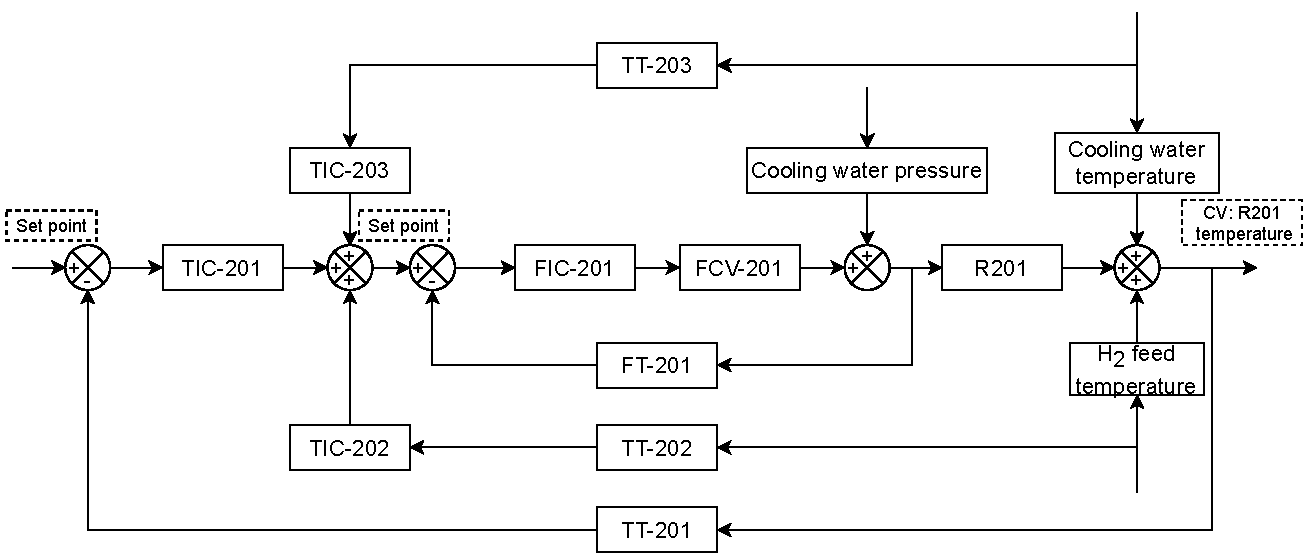
\includegraphics[width=0.8\linewidth]{chapters/4-operation-control/4-Figures/R201-TC.pdf}
    \caption{Temperature control loop for reactor R201}
    \label{fig:R201-TC}
\end{figure}

\subsubsection{Reactor R201 pressure control} %R201-PC
\begin{wrapfigure}{r}{0.6\linewidth}
    \centering
    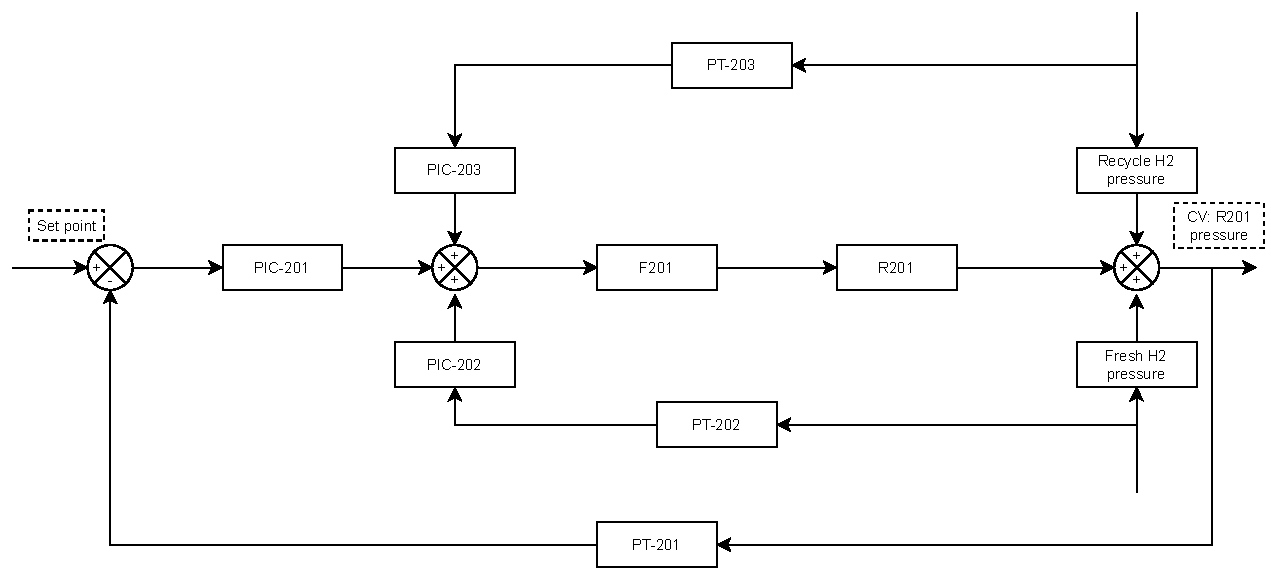
\includegraphics[width=\linewidth]{chapters/4-operation-control/4-Figures/R201-PC.pdf}
    \caption{Pressure control loop for reactor R201}
    \label{fig:R201-PC}
\end{wrapfigure}
The ONT reduction reactor is operated under pressure at 5 atm. To maintain this optimum operating condition and most importantly reduce the risk of overpressure and explosion, the pressure within the reactor is closely monitored and controlled. The manipulated variable is the pressure of the gas feed to the reactor, which should also be maintained at 5 atm. A pressure control is installed onto the fresh hydrogen feed line. To account for disturbances in the pressure of the recycled gas and in the pressure of the hydrogen coming from a pressurized storage tank, feedforward control was added. 



\subsubsection{Ratio control of reactants} %R201-CC
Ratio control is a special type of feedforward control whose objective is to maintain a specified ratio between two process streams. It is used in Nitroma's plant to maintain a stoichiometric ratio of reactants to reactor R201. Two different control schemes are proposed by \textcite{}: for both, one of the stream is treated as a disturbance which is measured by a transmitter. In the most classic scheme, the ratio of signals from the two transmitters are sent to a ratio controller acting on a flow control valve. In the more advance control scheme, the measurement from the disturbance stream is fed into a ratio station which calculates what the 

\begin{figure}[H]
    \centering
    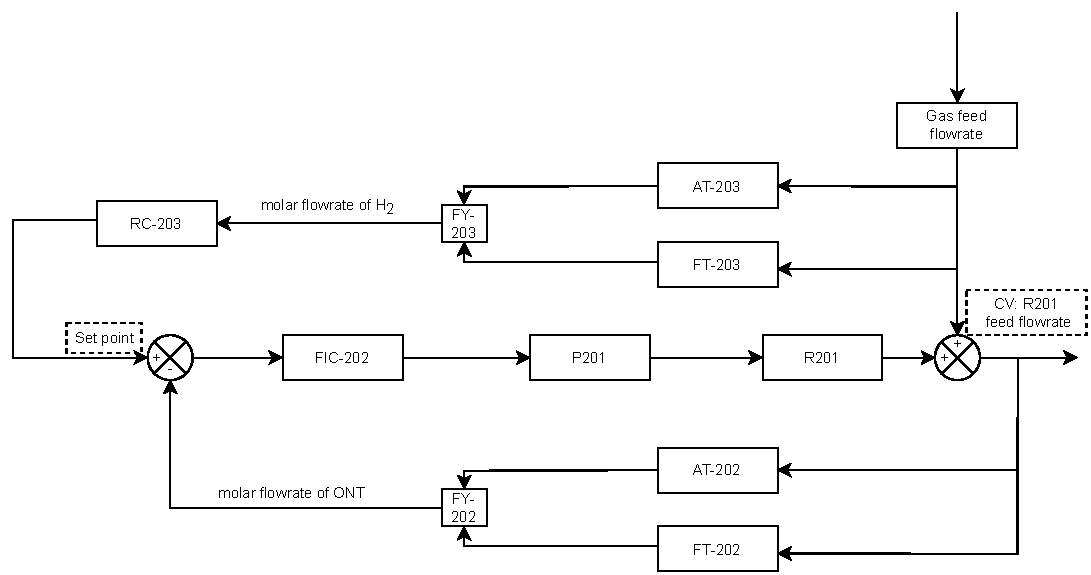
\includegraphics[width=0.8\linewidth]{chapters/4-operation-control/4-Figures/R201-FC.pdf}
    \caption{Ratio control of reactants to reactor R201}
    \label{fig:R201-FC}
\end{figure} 


\subsubsection{Hydrogen recycle control}%V202-CC
\begin{wrapfigure}{r}{0.6\linewidth}
    \centering
    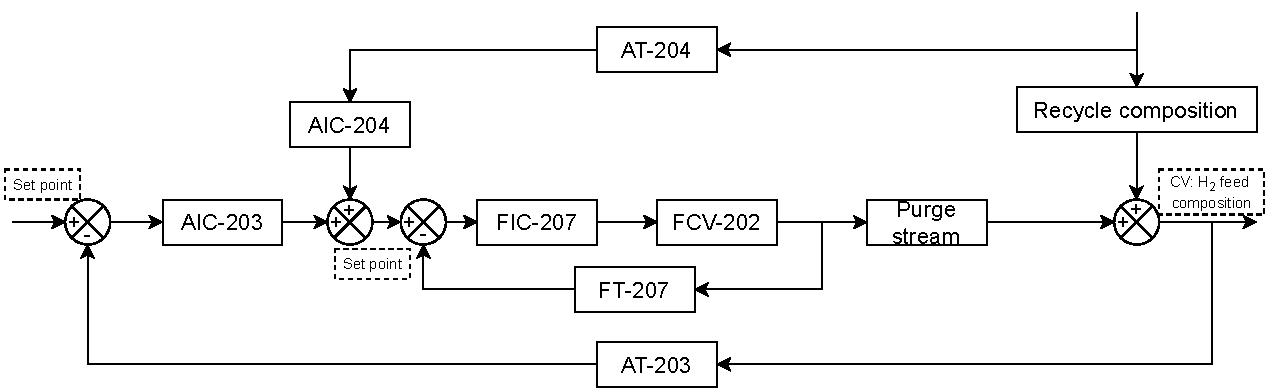
\includegraphics[width=\linewidth]{chapters/4-operation-control/4-Figures/V202-CC.pdf}
    \caption{Gas feed composition control with recycle purge}
    \label{fig:V202-CC}
\end{wrapfigure}
The composition of the gas feed to the reactor is controlled via the purge fraction of the gas recycle, composed of a mixture of unreacted hydrogen and vaporised methanol solvent. A master composition controller infers a set point to a slave flow controller which acts on a flow control valve installed in the recycle purge stream. To know how much recycled gas should be purged to meet the required gas feed composition, the recycle composition is analysed and accounted for with feedforward control. 



\subsubsection{Reactor R201 level control} % R201-LC
The liquid level at the bottom of the reactor operating co-currently and with downhill flows is controlled with a cascaded feedback loop. The master level controller infers a set point to the slave flow control which acts on the flow control valve installed on the reactor outlet. By increasing the liquid take-off from the reactor, the level of the liquid hold-up at the bottom of the reactor will reduce.


\subsubsection{Hydrogen feed flowrate control} %R201-HFC
The flowrate of hydrogen feed to the reactor R201 is adjusted by the speed of the fan F201. A feedback control loop acts on the motor of the fan to change this power and thus the fan speed according to the gas flowrate measured downstream of the fan with a flow transmitter. The main identified disturbances are the pressure of the fresh hydrogen and the flowrate of recycled gas. Those disturbances are already accounted for in the reactor pressure control loop and the hydrogen recycle control. 




\subsubsection{Reactor R201 feed temperature control}%H201 and H202-TC 
%no graph
The reactor gas and liquid feeds are heated by electric heaters, numbered respectively H201 and H202. Feedback control loops are installed to adjust the power of the electric heater to meet the required feed temperature. Feedforward control to account for disturbances in the temperature of the streams before entering the heaters was judged unnecessary since the electric heaters can quickly adjust the heat duty, usually in the order of seconds. This is one of the advantage of using electric heaters instead of heat exchangers with high or low  pressure steam.


\subsubsection{Distillation column S201 pressure control} %S201-PC
Pressure in distillation columns is one of the most important parameters to control as it not only affects the relative volatilities of the heavy and light keys, but also the shape of the vapour-liquid phase equilibrium curves which determine the compositions of the top and bottoms products. The manipulated variable for pressure control needs to be made carefully from several options, such as controlling the vapour flow that is vented from the reflux drum, condenser duty, reboiler duty, recirculation of cooling fluid in the condenser or addition of inerts. Controlling the vapour flow that is vented from the reflux drum is the simplest control to implement and usually provides the fastest response as the amount of gas holdup in the column directly affects its pressure. In addition, the vapour flow rate from the condenser is large, making it easier to effect a change in pressure from a small change in valve position. This avoids a situation where the flow control valve becomes saturated when mitigating a large disturbance to pressure. 
An optimal feedback control was designed with the vapour flowrate from the reflux drum as the manipulated variable. A pressure transmitter (PT-206) measures the pressure in the column, which is monitored by a pressure controller (PIC-206) that regulates a flow control valve (FCV-205) on the vent stream from the reflux.

%no graph
%\begin{figure}[H]
 %   \centering
  %  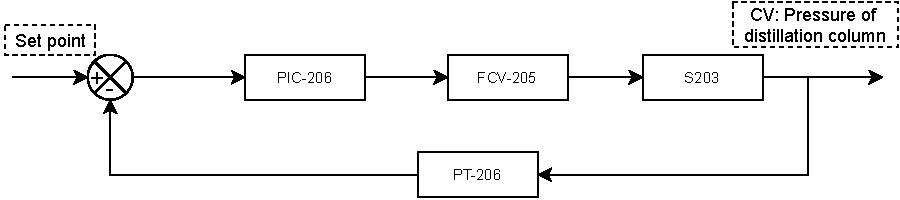
\includegraphics[width=\linewidth]{chapters/4-operation-control/4-Figures/S203-PC.pdf}
   % \caption{}
    %\label{fig:S203-PC}
%\end{figure}


\subsubsection{S201 feed pressure control} %V201-PC
To further ensure tight control of pressure in the column, a feedback control loop controls a pressure control valve on the feed to the column to minimise disturbances to the feed pressure of the column.

%no graph
%\begin{figure}[H]
 %   \centering
  %  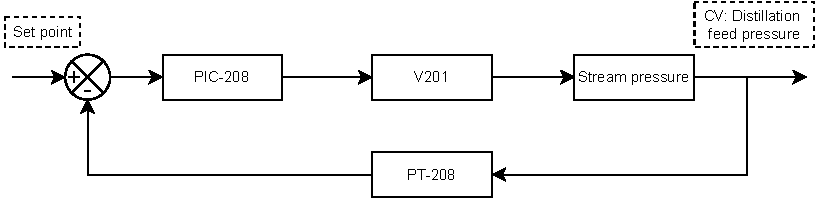
\includegraphics[width=\linewidth]{chapters/4-operation-control/4-Figures/V201-PC.pdf}
   % \caption{}
    %\label{fig:V201-PC}
%\end{figure}


\subsubsection{Bottom stream composition control} %S201-CC
\begin{wrapfigure}{r}{0.6\linewidth}
    \centering
    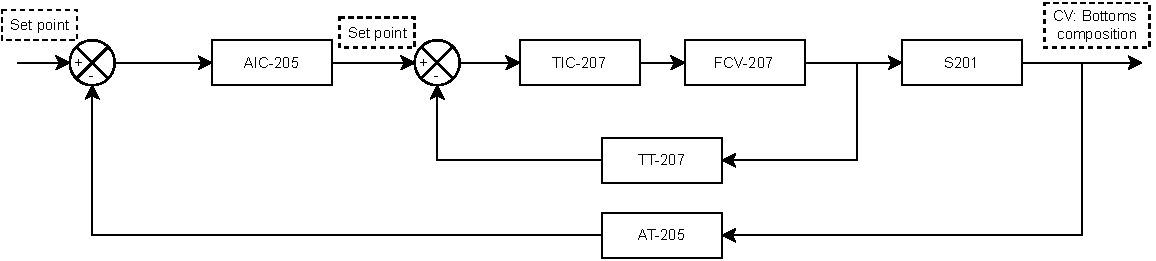
\includegraphics[width=\linewidth]{chapters/4-operation-control/4-Figures/S201-CC.pdf}
    \caption{}
    \label{fig:S201-CC}
\end{wrapfigure}
A composition control loop in the distillation column is also necessary to ensure a high recovery of o-toluidine. Since o-toluidine is found in the bottoms stream, reboiler duty was chosen as the manipulated variable in order to reduce the lag time of the controller. A composition analyser (AT-205) measures the concentration of o-toluidine in the bottoms stream and a composition controller (AIC-205) controls the reboiler duty by manipulating a flow control valve (FCV-207) on the saturated steam. 
A composition analyser was chosen to allow direct online measurements of the concentration of o-toluidine, one of the end products of our plant. However, composition analysers often have a slow dynamic response because of long measurement times. There would be delays in the controller response that would lead to a poor control of product quality. To mitigate this, the temperature of the column is used as an inferential measurement to control the product composition. Temperature sensors have quicker dynamic responses, and the temperature profile in the column directly affects product compositions. A calibration curve can be established using phase equilibrium data of methanol and o-toluidine to allow temperature to act as a proxy for composition control. An added benefit of controlling temperature is to also prevent accumulation of thermal energy in the column that would be a safety hazard. Figure \ref{fig:S201-CC} shows the temperature controller (TIC-207) that receives its setpoint from the master composition controller (AIC-205), and outputs a signal to the flow control valve FCV-207.




%\subsubsection{Distillation column S201 level control}
%The liquid level at the bottom of the distillation column S201 is an important inventory to control to prevent the reboiler from drying up. This would also result in weeping in the column and decreased performance. Since the reboiler duty is used for composition control, the most direct way of controlling the level is the bottoms flowrate out of the reboiler. Due to the reboiler being able to store a certain amount of liquid inventory, a lag between the response of the actuator and the level is expected. While in most cases a simple feedback controller is sufficient (see Figure \ref{fig:S203-LC}, experimental data would confirm if more advanced systems are needed to compensate for a large time delay. 

%\begin{figure}[H]
   % \centering
   % 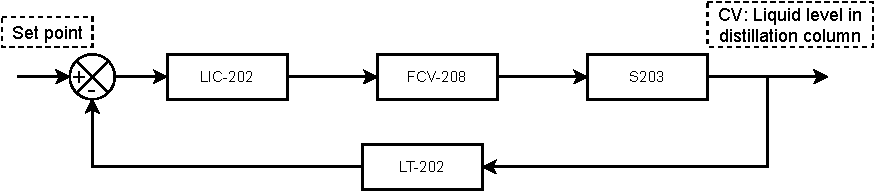
\includegraphics[width=\linewidth]{chapters/4-operation-control/4-Figures/S203-LC.pdf}
  %  \caption{}
  %  \label{fig:S203-LC}
%\end{figure}


\subsubsection{Reboiler H204 level control} %H204-LC
%no graph
The liquid level in the reboiler H204 is an important inventory to control to prevent the reboiler from drying up. This would also result in weeping (a lack of vapour flow) in the column and decreased performance of the separation unit. Since the reboiler duty is used for composition control, the most direct way of controlling the level is the bottoms flowrate out of the reboiler. A simple feedback controller is used. 

\subsubsection{Reflux drum S204 level control}%S204-LC
Similar to the level control in the reboiler, controlling the level of liquid in the reflux drum is required for stable operation of the column. Letting the drum run dry would lead to no reflux returning to the column, which would affect the separation efficiency of the light and heavy components. The manipulated variable for the liquid level was chosen to be the tops product flowrate, as it was desirable to maintain a constant reflux ratio to the column in order that the energy required to achieve the desired degree of separation would remain constant. In order to account for disturbances to the column performance because of variations in feed flowrate, a feedforward controller was implemented to adjust the tops product flowrate based on the feed flowrate. This prevents material and energy buildup in the column. 


\subsubsection{Condenser H203 heat duty control}%H203-TC
\begin{wrapfigure}{r}{0.6\linewidth}
    \centering
    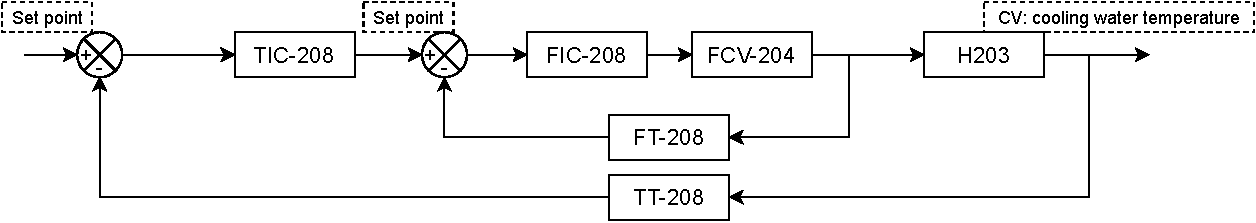
\includegraphics[width=\linewidth]{chapters/4-operation-control/4-Figures/H203-TC.pdf}
    \caption{}
    \label{fig:S203C-TC}
\end{wrapfigure}
The condenser in a distillation column provides cooling to condense the vapour exiting from the top of the column. It is usually desirable to operate the condenser at maximum duty, as reflux to the column has to be in a liquid state. Thus it is important to ensure that any disturbances to the cooling water flowrate and temperature are mitigated with a control loop. A cascade control was proposed, with the slower temperature loop as the master control and flowrate as the slave (see Figure \ref{fig:S203C-TC}). This way, any disturbances in the flow can be quickly rectified by the flow controller (FIC-208), while the temperature controller (TIC-208) gradually modifies the overall setpoint for the flow to account for disturbances in temperature.

\subsection{Process and control loop interactions}
The established controls so far have assumed that one manipulated variable (mv) only affects one control variable (cv). In reality, it is likely that manipulating one variable will affect multiple controlled variables and we have a multiple-input, multiple-output (MIMO) system. For example, reducing reboiler duty would directly reduce column temperature because of reduced vapour flow, but this would also indirectly affect the temperature of the reflux that gets sent back to the column. 

In principle, good control of MIMO systems requires quantitative information about the dynamics of the system to choose the best mv-cv pairings and minimise control loop interactions. This was beyond the scope of this report, however a more advanced controller design would be feasible once experimental work on a pilot scale plant was carried out to determine the dynamic responses of various mvs to the cvs.

\subsubsection{Relative Gain Array}

\begin{wrapfigure}{r}{0.5\linewidth}
    \centering
    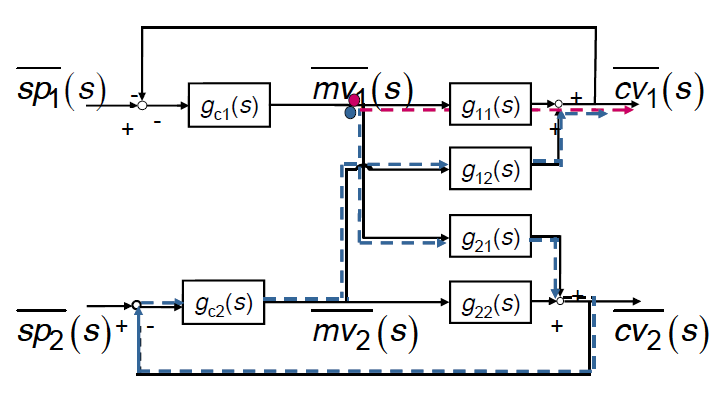
\includegraphics[width=\linewidth]{chapters/4-operation-control/4-Figures/RGA-Thornhill-2013.png}
    \caption{Block diagram showing the effect of changing mv1 on cv1. The direct effect of mv1 is shown via the pink path, while the indirect effect of mv1 is shown via the blue path. Image adapted from \textcite{}}
    \label{fig:RGA-block-di}
\end{wrapfigure}

The Relative Gain Array (RGA) method decides the best control loop pairings based on the steady state gains of each mv-cv pair. This is determined by the relative gain, which is the ratio of the direct effect to the total effect of changing mv on cv (see Figure \ref{fig:RGA-block-di}). A good controller is one with the highest relative gain, because it means that the direct effect dominates over the indirect effect which allows for the fastest controller response and minimal disturbance to other cvs. However, while RGA analysis does suggest the best loop pairings, it does not present a solution to interactions between control loops due to the indirect effects of mvs on cvs.

\subsubsection{Controller Decoupling}
Decoupling controllers can be designed to reduce loop pairings which have significant indirect effects on other controlled variables. For example, the indirect effect of reboiler duty on column temperature as a consequence of changes to the reflux is likely to be significant. Significant interactions from different mv on a cv will be apparent if the relative gains of the particular cv are much lower than 1. 

Decoupling controllers aim to cancel the indirect effect on a cv by sending a compensating signal through the direct path. Their design requires knowledge about the dynamic behaviour of the process, in order to deduce the transfer functions between each mv-cv pairing. This can be obtained experimentally, after which the controller transfer function needs to give an equal but opposite effect to the indirect effect. In Figure \ref{fig:RGA-block-di}, controller gDC1(s) is a detuning controller to mitigate the indirect effect of mv1 on cv1 (blue path), with transfer function according to Equation \ref{eqn:detuning}.

\begin{equation}
\label{eqn:detuning}
g_{DC1}(s)=-\frac{g_{12}(s)}{g_{11}(s)}
\end{equation}

% relative gain equation
\begin{comment}
\begin{equation}
\label{eqn:relative-gain}
\lambda_{ij}=\frac{(\partial y_i / \partial u_j)_u}{(\partial y_i / \partial u_j)_y}=\frac{open-loop\;gain}{closed-loop\;gain}
\end{equation}
\end{comment}
% end comment


\subsection{Safety design} %mention HAZOP recommendations

\subsubsection{Alarms and emergency trips strategy}

\subsubsection{Alarms and safety interlocks design}

\subsubsection{Recommendations from LOPA} %Stephen
%link to safety
From the layers of protection analysis in the Safety Report, it was determined that overpressure of reactor R201 was a major hazard and that aside from the existing executive alarm and interlock, an additional safety instrumented function (SIF) with a SIL-3 rating was required. To improve the safe operation of the plant, a two-out-of-three logic system (2oo3) was designed. Three independent pressure transmitters (PT-214a,b,c) measure reactor pressure, and only send a signal to the pressure controller PIC-214 if at least two pressure readings indicate a serious overpressure (>6atm). The controller will process a high pressure signal and increase the outlet gas flowrate through two flow control valves (FCV-209 and FCV-210) which are maintained regularly. The redundancies in transmitters and actuators reduce the risk of a mechanical or electrical failure rendering the SIF inoperable, thus guaranteeing a SIL-3 rating. As a final layer of protection, a pressure relief valve was installed and set to burst at the critical pressure of 7.5atm.